\documentclass[english,floatsintext,man]{apa6}

\usepackage{amssymb,amsmath}
\usepackage{ifxetex,ifluatex}
\usepackage{fixltx2e} % provides \textsubscript
\ifnum 0\ifxetex 1\fi\ifluatex 1\fi=0 % if pdftex
  \usepackage[T1]{fontenc}
  \usepackage[utf8]{inputenc}
\else % if luatex or xelatex
  \ifxetex
    \usepackage{mathspec}
    \usepackage{xltxtra,xunicode}
  \else
    \usepackage{fontspec}
  \fi
  \defaultfontfeatures{Mapping=tex-text,Scale=MatchLowercase}
  \newcommand{\euro}{€}
\fi
% use upquote if available, for straight quotes in verbatim environments
\IfFileExists{upquote.sty}{\usepackage{upquote}}{}
% use microtype if available
\IfFileExists{microtype.sty}{\usepackage{microtype}}{}

% Table formatting
\usepackage{longtable, booktabs}
\usepackage{lscape}
% \usepackage[counterclockwise]{rotating}   % Landscape page setup for large tables
\usepackage{multirow}		% Table styling
\usepackage{tabularx}		% Control Column width
\usepackage[flushleft]{threeparttable}	% Allows for three part tables with a specified notes section
\usepackage{threeparttablex}            % Lets threeparttable work with longtable

% Create new environments so endfloat can handle them
% \newenvironment{ltable}
%   {\begin{landscape}\begin{center}\begin{threeparttable}}
%   {\end{threeparttable}\end{center}\end{landscape}}

\newenvironment{lltable}
  {\begin{landscape}\begin{center}\begin{ThreePartTable}}
  {\end{ThreePartTable}\end{center}\end{landscape}}




% The following enables adjusting longtable caption width to table width
% Solution found at http://golatex.de/longtable-mit-caption-so-breit-wie-die-tabelle-t15767.html
\makeatletter
\newcommand\LastLTentrywidth{1em}
\newlength\longtablewidth
\setlength{\longtablewidth}{1in}
\newcommand\getlongtablewidth{%
 \begingroup
  \ifcsname LT@\roman{LT@tables}\endcsname
  \global\longtablewidth=0pt
  \renewcommand\LT@entry[2]{\global\advance\longtablewidth by ##2\relax\gdef\LastLTentrywidth{##2}}%
  \@nameuse{LT@\roman{LT@tables}}%
  \fi
\endgroup}


  \usepackage{graphicx}
  \makeatletter
  \def\maxwidth{\ifdim\Gin@nat@width>\linewidth\linewidth\else\Gin@nat@width\fi}
  \def\maxheight{\ifdim\Gin@nat@height>\textheight\textheight\else\Gin@nat@height\fi}
  \makeatother
  % Scale images if necessary, so that they will not overflow the page
  % margins by default, and it is still possible to overwrite the defaults
  % using explicit options in \includegraphics[width, height, ...]{}
  \setkeys{Gin}{width=\maxwidth,height=\maxheight,keepaspectratio}
\ifxetex
  \usepackage[setpagesize=false, % page size defined by xetex
              unicode=false, % unicode breaks when used with xetex
              xetex]{hyperref}
\else
  \usepackage[unicode=true]{hyperref}
\fi
\hypersetup{breaklinks=true,
            pdfauthor={},
            pdftitle={A thorough evaluation of the Language Environment Analysis (LENATM) system},
            colorlinks=true,
            citecolor=blue,
            urlcolor=blue,
            linkcolor=black,
            pdfborder={0 0 0}}
\urlstyle{same}  % don't use monospace font for urls

\setlength{\parindent}{0pt}
%\setlength{\parskip}{0pt plus 0pt minus 0pt}

\setlength{\emergencystretch}{3em}  % prevent overfull lines

\ifxetex
  \usepackage{polyglossia}
  \setmainlanguage{}
\else
  \usepackage[english]{babel}
\fi

% Manuscript styling
\captionsetup{font=singlespacing,justification=justified}
\usepackage{csquotes}
\usepackage{upgreek}



\usepackage{tikz} % Variable definition to generate author note

% fix for \tightlist problem in pandoc 1.14
\providecommand{\tightlist}{%
  \setlength{\itemsep}{0pt}\setlength{\parskip}{0pt}}

% Essential manuscript parts
  \title{A thorough evaluation of the Language Environment Analysis (LENATM)
system}

  \shorttitle{IN PREP - LENA EVAL}


  \author{many\textsuperscript{1}}

  % \def\affdep{{""}}%
  % \def\affcity{{""}}%

  \affiliation{
    \vspace{0.5cm}
          \textsuperscript{1}   }

  \authornote{
    Correspondence concerning this article should be addressed to many, .
    E-mail:
  }


  \abstract{In the previous decade, dozens of studies involving thousands of
children across several research disciplines have made use of a combined
daylong audio-recorder and automated algorithmic analysis called the
LENA system, which aims to assess children's language environment.
However, validation of the system lags behind its growing importance in
the research domain. Here we assess LENA accuracy across its key outcome
measures: speaker classification, adult word counts, child vocalization
counts, and conversational turn counts. Our assessment is based on
manual (LENA-output naive) random and period sampling, in (a)
populations similar to LENAs original training data from North American
English-learning children, (b) another dialect of English (UK), and (c)
in a different language and socio-cultural setting (rural Bolivia). We
find reasonably high accuracy across some measures, with more
problematic levels of performance across others. We find little
difference in accuracy as a function of dialect, language, or
socio-cultural setting. Whether LENA results are ``good enough'' for a
given research, educational, or clinical application depends largely on
the specifics at hand; we conclude with a set of recommendations to help
researchers make this determination for their goals.}
  




\begin{document}

\maketitle

\setcounter{secnumdepth}{0}



While nearly all humans eventually become competent users of their
language(s), documenting the experiential context of early acquisition
is crucial for both theoretical and applied reasons. Regarding theory,
there are many open questions about what kinds of experiences and
interactions are necessary, sufficient, or optimal for supporting
language development. Moreover, the ability to accurately and quickly
assess an infant's state of development at a given point in time is of
central importance for clinical purposes, both for children with known
risks of language delays and disorders, and those who might not be
identified based on risk factors. Reliable assessments are also crucial
for measuring intervention efficacy.

One approach that has been making its way into the mainstream literature
across applied and basic research on language and cognition relies on
day-long recordings gathered with LENA(R) products (e.g.~Greenwood et
al, 2011; Oller et al 20 2010; Gilkerson et al 2017, inter alia),
analyzed by LENA's automated, closed-source algorithms. As we summarize
below, this approach has many advantages, which may explain its
expanding popularity. While dozens of papers over the past decade have
used LENA's automated output, only a handful include validity estimates
{[}e.g.~Weisleder \& Fenald 2013; Zimmerman et al 2009, d'Apice et al
2019{]}, even fewer where validity estimation was the primary focus of
the paper (e.g.~Ganek \& Eriks-Brophy, Bulgarelli \& Bergelson, in press
@ BRM, Lehet Dilley Houston; for a fuller report, see Cristia et al,
under review). As a result, few studies report sufficient details about
validation accuracy for one or more metrics, limiting systematic review
or meta-analytic assessment (Cristia et al., under review).

The work undertaken thus far also has some limitations, which are
described further in the \enquote{Previous Validation} section below,
and mentioned briefly next. First, many validations or evaluations of
LENA omit analysis of the less-directly \enquote{relevant} categories of
input like noise, silence, or overlap. Second, many LENA evaluations
rely on LENA's own output as a starting point to either select portions
of the file for manual annotation, or use its segmentation into
talker-turns as the unit of analysis (without conducting independent
segmentation). Both decisions can lead to inflated accuracy estimates.
Here we endeavor to conduct an evaluation that is fully independent of
the LENA algorithms automated output assessment, permitting a
systematic, extensive, and independent evaluation of the key automated
metrics provided by this system. Summarily, we report the LENA(R)
algorithms' performance based on random or periodic sampling from a set
of recordings, which (as detailed and argued below) is preferable to
other types of sampling. We conduct our analysis on (a) a sample of
children similar to the LENA(R) training set (i.e.~infants and toddlers,
growing up in North American English-speaking homes, {[}LTR-06-2{]}) (b)
check for generalization to a different dialect (UK English); and (c)
extend our analysis to a different language and setting
(Tsimane'-speaking homes in rural Bolivia).

\subsubsection{Brief introduction to LENA(R)
products}\label{brief-introduction-to-lenar-products}

The LENA(R) system consists of a hardware component (a lightweight,
sturdy, and easy-to-use recording device worn by a child in specialized
clothing) and a suite of proprietary computer programs designed to
provide automated quantitative analyses of the auditory environment and
the child's own vocalizations.

The LENA software was developed over an extensive corpus of full day
audio recordings from a child's perspective using their patented
recording hardware {[}Xu et al, 2009{]}. The original dataset included
over 65,000 hours of recording across 329 American English-speaking
families chosen for diversity in child age (1-42 months) and
socio-economic status {[}LTR-6-2{]}. From these recordings, half-hour
selections from 309 recordings were transcribed and annotated for the
purpose of developing the algorithm, and an additional 60 minutes from
each of 70 recordings were transcribed and annotated for testing the
result {[}ibid{]}.

The resulting LENA software takes each audio recording and processes it
incrementally in short windows, extracting a variety of acoustic
features which are used to classify the audio stream into segments of at
least 600 ms in length (or longer for some of the categories) using a
Minimum Duration Gaussian Mixture Model (MDGMM, {[}Xu et al, 2008{]}).
Silence may be included to \enquote{pad} segments to this minimum
duration. The segments are classified according to a set of broad
speaker classifications - Male Adult, Female Adult, \enquote{Key} Child
(i.e.~the one wearing the recorder) and Other Child - and non-speaker
classifications - Noise, Television (including any electronics), Overlap
(speech overlapped with other speech or nonspeech sounds), and Silence
(SIL). With the exception of Silence, these classifications are then
passed through a further likelihood test and labeled as \enquote{Near}
(high probability) or \enquote{Far} (low probability), yielding the
following classes: MAN/MAF, FAN/FAF, CHN/CHF, CXN/CXF, NON/NOF, TVN/TVF,
OLN/OLF. Given the large number of acronyms and labels of various kinds,
we provide a listing of relevant LENA abbreviations on Table xx; in what
follows, we highlight the specific labels that we evaluate in the
present work in bold.

After this broad speaker classification step, Female or Male Adult
\enquote{Near} segments (FAN and MAN) are further processed using an
adaptation of the Sphinx Phone Decoder {[}Lamere et al, 2003{]} in order
to form an automated estimate of the number of words in each segment
(adult word count, or \textbf{AWC}). Key Child (CHN) segments are
further processed to sub-classify into vegetative noises (VEG), crying
(CRY), and speech-like vocalization (VOC). LENA provides the count
(child vocalization count, or CVC) and duration of these VOC
sub-segments. A further metric, Conversational turn counts (CTC),
reflects the number of alternations between an adult and the key child
(or vice versa), bounded by 5 s of non-speech.

Table xx. A partial listing of common LENA abbreviations and their
meanings.

\subsubsection{Previous validation work}\label{previous-validation-work}

A recent systematic review (Cristia, Bulgarelli, \& Bergelson,
submitted) found 23 papers, containing 28 studies, reporting on the
accuracy of LENA's labels and derived metrics (AWC, CVC, CTC). They
conclude there are \enquote{reasonably good results {[}overall{]}: over
61\% for recall and precision based on 11-12 non-independent studies;
correlations for AWC mean r=.79, on n=11, with a mean RER{[}Relative
Error Rate{]}=10\% on n=11; CVC mean r=.76, n=5, with a mean RER=1\% on
n=5. The exception to this general trend towards good performance was
CTC, with a mean r=.31, n=5, RER=-64\% on n=2.}

While this systematic review sought to take stock of the current
literature using LENA reportings, there were several limitations that
make it likely that these measures do not provide a full or fair picture
of LENA output accuracy. First, for the majority of included studies,
the validity report was not fully evaluated by peer review. Even if the
study may have appeared in a peer-reviewed report, the LENA validation
was often a secondary goal to support a different research objective,
and therefore often lacked methodological details or even full results.
For instance, Seidl et al. report on validation of LENA labels among
children at familial risk for autism in a short appendix to the journal;
in this Appendix, only confusions between female adult and child are
mentioned -- suggesting that confusions between key child and any other
category (other child, male adult, silence, etc.) were ignored rather
than counted as an error. While this approach may be reasonable for a
given study's goals, it has the undesirable side effect of reducing the
granularity of our understanding. Second, previous studies typically did
not take silence, noise, or overlap into account in the reported
confusion matrices or other accuracy measures, particularly within
segments. That is, if a LENA segment labeled \enquote{key child}
contained one second of silence and two seconds of speech, the full
three second clip was often tagged as \enquote{correct} though it was
only 67\% correct, leading to an overestimation of the accuracy of the
\enquote{key child} label.

Third, a majority of previous validation studies used the LENA output
itself to select the sections that would be annotated for validation (in
Cristia et al., subm, this held for 14/25 studies that specified the
method of selection). For instance, clips may have been selected for
manual annotation on the basis of high AWC and/or CTC according to the
algorithm. This unfortunately leads to biased sampling: Since LENA only
counts words within FAN and MAN segments and conversational turns
involving FAN/MAN alternations with CHN in close proximity, high AWC or
CTC can only occur in sections of the recording that are \enquote{clean}
enough for the algorithm to parse; otherwise, most of the section would
have been classified as overlap (OLN), which does not count towards AWC
or CTC. This would tend to bias these reports toward a higher level of
accuracy than would be obtained overall across the full recording.

Forth, previous validation work has typically focused on a single
corpus, participant population, age range, and language. As a result, it
is difficult to assess whether a numerical difference in accuracy found
across two papers is statistically significant. Even if this difference
is large, it is challenging to decide whether this is due to a
difference in the way the corpus was constituted and annotated, on how
LENA fares with that population, age range, and language.

\subsubsection{The present work}\label{the-present-work}

We sought to assess the validity of LENA's metrics through an approach
that complements the preceding literature (including our own work).
Specifically, we report an evaluation of all speech labels and some
non-speech labels of LENA (silence (SIL), overlap near (OLN), overlap
far (OLF)), as well as LENA's key derived metrics: adult word count
(AWC), conversational turn count (CTC), and child vocalization count
(CVC). We aim to address several of the potential limitations
highlighted above.

First, to maximally avoid potential bias in our annotations, we used
random or periodic sampling (detailed below) to choose which sections of
daylong recordings to annotate, and did not give annotaters access to
the LENA output. Second, to allow assessment of the accuracy of the
segmentation itself as well as categorical labeling, evaluation is done
at the level of 10 ms frames. This will allow us to capture a much
finer-grained representation of the auditory environment (i.e.~if LENA
classified a 2 s audio segment as FAN, but .8 s of this was actually
non-speech noise, LENA would be credited only for the proportion that
was correct).

Third, to gain traction on generalizability rather than focusing on a
single sample that either mirrors or diverges from LENAs original
population, we include five corpora. Three corpora based on the same
population, language, and dialect LENA was established with; a fourth
corpus that allows an extension to a different dialect of English; and a
fifth corpus that is an extension to a totally different recording
condition (a rural setting, with large families and many children
present, in a different language). The age range also varies a great
deal, particularly in this last corpus.

Finally, the present study relies on a collaborative annotation effort
across several labs. Critically, this means that we can \enquote{fairly}
compare annotations across our corpora: annotation decisions were either
identical or comparable, and all analyses were identical. This allows us
to more readily answer questions regarding differences in reliability as
a function of e.g.~child age and language.

\subsection{Methods}\label{methods}

\subsubsection{Corpora}\label{corpora}

The data for the evaluation comes from two different projects. The
largest one is the ACLEW project (Bergelson et al., 2017b Databrary
volume; Soderstrom et al AMPPS under review); in this paper we focus on
four different corpora of child daylong recordings that have been pooled
together, sampled, and annotated in a coordinated manner. These four
corpora are: the Bergelson corpus (\enquote{BER}) from US English
families from the upstate New York area (Bergelson, 2016), the LuCiD
Language 0--5 corpus (\enquote{L05}) consisting of English-speaking
families from Northwest England (Rowland et al., 2018), the McDivitt and
Winnipeg corpora ( \enquote{MCD}) of Canadian English families (McDivitt
\& Soderstrom, 2016), and the Warlaumont corpus (\enquote{WAR}) of US
English from Merced, California (Warlaumont et al., 2016). Some
recordings in BER, and all recordings in MCD and WAR are available from
HomeBank repository (VanDam et al., 2016). The second project contains a
single corpus collected from Tsimane' speaking families in Bolivia
(Scaff et al., in prep.; here \enquote{TSI}).

Key properties of the five corpora are summarized in Table 2. Each
corpus consists of daylong (4--16 hour) at-home recordings; each corpus
samples from a unique community. Corpora span languages and dialects;
socioeconomic environment varying both within and across corpora. In
each recording, the key child (\enquote{participant}) wears a LENA
recorder in a special vest throughout a normal day.

For the four ACLEW corpora, out of the 106 recorded participants,
daylong recordings from 10 infants from each corpus were chosen for
manual annotation, selected to represent a diversity of ages (0--36
months) and socio-economic contexts. In the SOD corpus, sensitive
information was found in one of the files, and thus one child needed to
be excluded. The tenth day for this corpus was a second day by one of
the 9 included children. From each daylong file, fifteen 2-minute
non-overlapping audio (with a 5-minute context window) were randomly
sampled from the entire daylong timeline for manual annotation. This 30
minute sample corresponded to approximately 1 minute of annotated speech
per key child (collapsing across all speaker categories).

The TSI corpus consisted of 1-2 daylong recordings from 12 infants, out
of the 25 recorded from field work that year; the other 13 had been
recorded using other devices (not the LENA DLP). From these daylong
files, 1-minute segments were sampled in a period fashion. That is, for
each day, we skipped the first 33 minutes to allow the family to
acclimate to the recorder, and then extracted 1 minute (with a 5-minute
context window) every 60 minutes, until the end of the recording was
reached. This resulted in 4 to 16 minutes of manually annotated audio
per child per recording (mean = 12.64 minutes), and an average of 3
minutes of speech per key child (collapsing across all speaker
categories).

We chose to sample 1 or 2 minutes at a time (Tsimane, and ACLEW corpora,
respectively) because conversations are likely to be bursty (Goh \&
Barbasi; cf.~Slone et al Fausey et al ICIS18 session). That is, it is
likely the case that speech is not produced at a periodic rate (e.g.,
one phrase every 20 seconds), but rather it occurs in bursts (a
conversation is followed by a long period of silence between the
conversational partners, followed by another bout of conversation,
perhaps with different interlocutors, followed by silence, and so on).
In this context, imagine that you sample a 5-second stretch. If you find
speech in that stretch, then it is likely you have by chance fallen on a
conversation bout; if you do not find speech, then you have likely found
a silence bout. If you were to extend that selection out to several
minutes, then it is likely that you will simply add more material from
the same type (i.e.~conversation bout or silence bout). As a result, any
sampling method that favors medium-sized stretches (5-15 minutes) will
tend to end up with samples that are internally homogeneous (throughout
the 5 minutes, there is a conversation), but highly heterogeneous as a
collection if sampling is random throughout the day. This in turn would
lead to artificially high correlations between LENA and human metrics in
all dependent variables (e.g., since probably little speech, fewer
turns, and fewer child vocalizations will be found in silent bouts and
more in conversational ones). Thus, our strategy of sampling
randomly/periodically and in short stretches is more likely to represent
both conversational and short bouts, and to capture finer-grained
variation in speech quantity.

In the 5 corpora, the 1- or 2-min samples were annotated for all
hearable utterance boundaries and talker ID. In ACLEW corpora
\footnote{see Casillas et al., 2017a, 2017b for the general annotation protocol, and Soderstrom et al., submitted to AMPPS, for an introduction to the databases},
talker IDs reflected unique individual talkers, but were coded in such a
way to readily allow mapping onto LENAs talker categories (e.g.~key
child, other children, female adult, male adult). In the TSI corpus,
only the key child and one female adult whose voice recurred throughout
the day were individually identified, with all other talkers being
classified on the basis of broad age and sex into male adult, female
adult, and other children. The ACLEW datasets had other coding levels
which will not be discussed here.

\subsubsection{Processing}\label{processing}

Several different time units are needed to clarify how different metrics
are calculated (see Figure XX). Clips refer to the 1- or 2-minute
samples extracted from recordings. This is the basic unit at which child
vocalization counts and conversational turn counts can be established.
In addition, since most previous work evaluating adult word counts did
so at the clip level, we do so here as well.

\begin{figure}
\centering
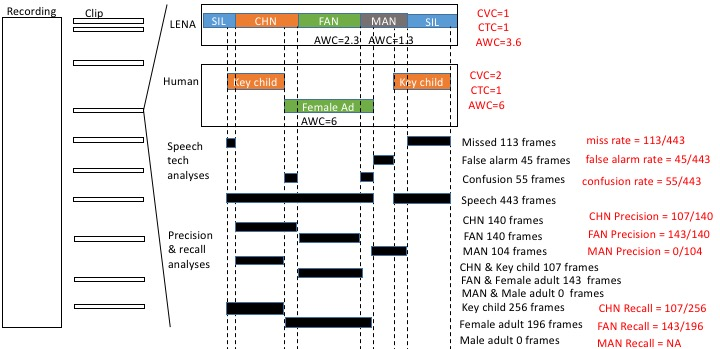
\includegraphics{fig_levels.jpg}
\caption{Levels at which performance is evaluated.}
\end{figure}

The other metrics require a more detailed explanation, conveyed
graphically in Figure XX. The stretch of time that has been assigned to
a speech or non-speech category by LENA is a segment. In one clip, there
may be just one long segment (e.g., the whole clip has been assigned to
Silence by LENA); or there may be more (e.g., the first 5 seconds are
attributed to the key child, then there is a 50-second Silence segment,
and the final 5 seconds are attributed to a Female Adult). In LENA's
automated analysis, only one of these categories may be active at a
given point in time. In contrast, we typically speak of utterances or
vocalizations to refer to stretches of speech detected by humans and
assigned to different talkers. Again, clips may have zero or more
utterances. Unlike LENA, however, a given point in time may be
associated with multiple speakers. Given that there need not be a
one-to-one correspondence between LENA segments and human utterances, we
need to define smaller time units that can be used to check for
agreement. In this paper, we use 10 ms frames. This is the basic time
unit used for all classification accuracy estimations, which are
introduced in more detail in the next subsection.

\subsubsection{LENA classification
accuracy}\label{lena-classification-accuracy}

Our first goal was to establish LENA talker tag accuracy, particularly
for the four broad LENA talker categories (key child, other child,
female adult, male adult; or CHN, CXN, FAN, MAN), but taking into
account other categories (with some limitation on their interpretation).
We calculated accuracy in two complementary ways. First, we used three
frame-based, standard metrics of speech and talker segmentation to allow
direct comparison with other systems in the speech technology literature
(False Alarms, Misses, Confusion Rate). We also use Diarization Error
Rate, which is derived from the first three metrics; together these
provide a stringent and standard test of accuracy. Second, we used
frame-based precision and recall of each category to provide an
intuitive representation of the error patterns shown by this system. In
both cases, electronic voices were rare in the ACLEW annotations and not
coded at all (by design) in the Tsimane data, they were mapped onto
silence.

\paragraph{Speech and talker segmentation
metrics}\label{speech-and-talker-segmentation-metrics}

The original coding was converted using custom-written python scripts
into rttm format (REF), a text-based format indicating, for each
vocalization, its start time, duration, and speaker. This representation
was used in pyannote.metrics (REF) to compute four standard diarization
metrics: rate of false alarm for speech, rate of misses for speech, rate
of confusion between talkers, and the derived diarization error rate
(DER). These are calculated with the following formulas at the level of
each clip, where FA (false alarm) is the number of frames during which
there is no talk according to the human annotator but during which LENA
found some talk; M (miss) is the number of frames during which there is
talk according to the human annotator but during which LENA found no
talk; C (confusion) is the number of frames correctly classified as LENA
as containing talk, but whose voice type has not been correctly
identified (when the LENA model recognizes female adult speech where
there is male adult speech for instance), and T is the total number of
frames that contain talk according to the human annotation:

\begin{itemize}
\tightlist
\item
  false alarm rate = FA/T,
\item
  miss rate = M/T,
\item
  confusion rate = C/T,
\item
  DER = (FA+M+C)/T,
\end{itemize}

In the human annotation, there is no class representing overlapping
speech as such. For the sake of completeness and full comparison with
the LENA model, time where two or more different speech sources were
active at the same time, according to the human annotators, have been
mapped to the class \enquote{overlap} post hoc. This allows us to
compare this Overlap class to LENA's OLN (and, for the precision/recall
analysis introduced next, OLF) by the LENA model. Therefore, the
confusion rate is computed based on the matches in Table XX.

Table XX: Correspondances between LENA and our human annotation.
*Electronic voices were only annotated in the ACLEW dataset. Although
some Tsimane' families listen to the radio, radio speech was not
annotated in the TSI corpus.

Please remember that the overlap category is not defined the same way as
the LENA overlap category. For LENA, overlap between any two categories
falls within overlap -- i.e., CHN+TV would be counted towards overlap as
would FAN+FAN; whereas for us, only overlap between two talker
categories (e.g., key child and female adult) counts as overlap.
Similarly, the TVN is not equivalent to the electronic speech tag in the
ACLEW coding.

\paragraph{Precision and recall}\label{precision-and-recall}

This evaluation looks in more detail at the pattern of errors, by
assessing how LENA and human annotators agreed and disagreed. In both
precision and recall, the numerator is the intersection between a LENA
tag and a human tag (e.g., the number of frames that LENA classified as
CHN and the annotator classified as Key child; notice, there is no
constraint that these two categories by conceptually the same). The
denominator differs: To calculate precision, we divide that number by
the total number of frames attributed to a category by LENA, whereas for
recall, we divide by the total number of frames attributed to a category
by the human annotator.

\subsubsection{CVC and CTC evaluation}\label{cvc-and-ctc-evaluation}

From the human annotation, each vocalization by the key child counted
towards the total Child Vocalization Count (CVC) for a given clip. For
the Conversational Turn Count (CTC), a sequence of key child and any
adult (or vice versa) within 5 seconds counted towards the clip total
CTC.

\subsubsection{AWC evaluation}\label{awc-evaluation}

For the AWC portion of this evaluation, we could only use transcriptions
from the four ACLEW corpora, since the TSI corpus has not been
transcribed (and thus lacks word counts). In contrast, annotators for
the four ACLEW corpora were proficient in the language spoken in the
daylong recording, and transcribed all adult speech based using
canonical lexical forms (e.g. \enquote{wanna}, not \enquote{want to}) in
keeping with minCHAT format (MacWhinney).

Reference adult word counts were determined by counting all
unambiguously transcribed words spoken by adult talkers. This was
achieved by first discarding all non-lexical transcript entries such as
non-linguistic communicative sounds, paralinguistic markers, and markers
indicating incomprehensible speech. In addition, all utterances from the
key child and other children were omitted from the Adult Word Count. The
remaining orthographic entries separated by whitespaces were then
counted as gold standard target words for LENA to detect.

As for LENA word counts, the regions sampled for manual annotation were
not guaranteed to perfectly align with LENA utterances. Of all LENA
utterances overlapping with the annotated speech, 14\% had only partial
overlap with the annotations. To match LENA AWCs with the annotated word
counts, words from the partially overlapping LENA utterances were
included in proportion to the amount of overlap between the LENA turn
and the reference segment in question (e.g., if 10\% of a LENA-estimated
utterance was overlapping with a manually-annotated utterance, 10\% of
the total LENA AWC estimate for the given turn was included in the LENA
word count estimate for that reference segment).

\subsection{Results}\label{results}

Before starting, we provide some general observations based on the human
annotation. Silence is extremely common, constituting 79\% of the
frames. In fact, 45\% of clips contained no speech by any of the human
speaker types (according to the human annotators). As for speakers,
female adults make up 11\% of the frames, the child contributes to 4\%
of the frames, whereas male adult voices, other child voices, and
electronic voices are found in only 1\% of the frames each. Overlap
makes up the remaining 3\% of the frames. The following consequences
ensue: if frame-based accuracy is sought, a system that classifies every
frame as silence would be 79\% correct. This is of course not what we
want, but it indicates that systems adapted to this kind of speech
should tend to have low \enquote{false alarm} rates, i.e.~a preference
for being very conservative as to when there is speech. If the system
does say there is speech, then it had better say that this speech comes
from female adults, who provide a great majority of the speech. In
second place, it should be key child. Given that male adults and other
children are rare, a system that makes a lot of mistakes in these
categories may still have a good global performance, because these
categories are extremely rare.

\subsubsection{LENA classification accuracy: False alarms, misses,
confusion}\label{lena-classification-accuracy-false-alarms-misses-confusion}

Our first analysis is based on standard speech technology metrics, which
put errors in the perspective of how much speech there is. That is, if
10 frames are wrong in a file where there are 100 frames with speech,
this is a much smaller problem than if 10 frames are wrong in a file
where there is 1 frame with speech. In other words, these metrics should
be considered relative error metrics. One problem, however, emerges when
there is no speech whatsoever in a given file. In the speech technology
literature, this is never discussed, because most researchers working on
this are basing their analyses on files that have been selected to
contain speech (e.g., recorded in a meeting, or during a phone
conversation). We still wanted to take into account clips with no speech
inside because it is key for our research goals: We need systems that
can deal well with long stretches of silence, because we want to measure
how much speech children hear. Indeed, as mentioned above, 45\% of our
clips had no speech whatsoever. In these cases, the false alarm, miss,
and confusion rates are all undefined, because the denominator is zero.
In all likelihood, this leads to an overestimation of LENA's
performance, because potential false alarms in these files are not
counted against the system. It also occurred that there was just a
little speech; in this case, the denominator is very small, and
therefore the ratio for these two metrics ended up being a very large
number. To avoid such outliers having an undue impact on our report, we
present medians (rather than means).

There were, a priori, several ways of analyzing the data:

\begin{itemize}
\tightlist
\item
  collapsing near and far together (i.e., CHN and CHF were mapped onto a
  single CH category)
\item
  treating the near and far categories separately (i.e., CHN and CHF are
  both treated as \enquote{speakers}, but not the same one)
\item
  not considering TV as a speaker category, since it is conceptually not
  identical to the electronic voices detected by ACLEW human annotators;
  in this case, the gold annotations should also map electronic voices
  to non-speech or silence
\item
  not considering OLN as a speaker category, since it is not
  conceptually identical to the overlap derived from humans' annotating
  different speaker categories.
\end{itemize}

We thought the most informative decision would be to report on several
of these settings, albeit briefly. We start with the situation that
yields the best LENA performance: Electronic voices in the gold
annotation are mapped onto silence, so that the categories found in the
human annotation are FEM, MAL, CHI, OCH, and overlap; in the LENA
annotation, only CHN, FAN, MAN, and CXN are considered speakers (with
all far categories, TVN, and OLN all mapped onto silence). In this
setting, LENA's false alarm (i.e., saying that someone was speaking when
they were not) had a median of 12\%, whereas the miss rate had a median
of 49\%. The confusion rate, as mentioned above, is only calculated for
the correctly detected speech (i.e., not the speech that was missed,
which counts towards the miss rate, nor the speech that was falsely
identified, which is considered in the false alarm). The confusion rate
was very low, with a median of 10\%. These three metrics can be added
together into a single \enquote{diarization error rate}. The median
diarization error rate over the clips that had some speech was 79\%.

If electronic voices in the gold annotation are still mapped onto
silence and in the LENA annotation, CHN, FAN, MAN, CXN as well as OLN
are considered speakers (with all far categories as well as TVN mapped
onto silence), so that the human categories considered were CHI, FEM,
MAL, OCH, and overlap; and the LENA categories considered were CHN, FAN,
MAN, CXN, and OLN. In this setting, LENA's false alarm, missed, and
confusion rate medians were 33\%, 21\%, and 28\% respectively, for a
total median diarization error of 82\%. Performance likely degrades
because OLN is not picking up the same regions as the overlapping speech
found in the human annotations.

Next, we allowed the electronic voices segmented by humans, and TVN
among the LENA speaker categories, to be considered during the
evaluation (rather than mapping them all to non-speech or silence), so
that the human categories considered were CHI, FEM, MAL, OCH, overlap,
and electronic; and the LENA categories considered were CHN, FAN, MAN,
CXN, OLN, and TVN. LENA's false alarm, missed, and confusion rate
medians were 40\%, 18\%, and 30\% respectively, for a total median
diarization error of 88\%. Performance likely degrades because TVN is
not picking up the electronic speech segmented by ACLEW annotators.

Finally, we declared the maximum possible number of categories: The
human categories considered were still CHI, FEM, MAL, OCH, overlap, and
electronic; but the LENA categories considered were CHN, FAN, MAN, CXN,
OLN, TVN, CHF, FAF, MAF, CXF, OLF, TVF. LENA's false alarm, missed, and
confusion rate medians were 74\%, 7\%, and 41\% respectively, for a
total median diarization error of 122\%. Performance degrades because
everything is treated as speech, leading to huge apparent false alarm
rates.

\subsubsection{LENA classification accuracy: Precision and
recall}\label{lena-classification-accuracy-precision-and-recall}

By now, we have established that the best performance (when
\enquote{far} labels such as CHF and OLF are mapped onto silence, as are
TVN and OLN), the overall relative diarization error rate is about 79\%,
due mainly to missing speech (49\%), with false alarms (12\%) and
confusion between talker categories (10\%) constituting a relatively
small proportion of errors. However, this metric may not capture what
our readers are interested in, for two reasons. First, this metric gives
more importance to correctly classifying segments as speech versus
non-speech (False alarms + misses) than confusing talkers (confusion).
Second, many LENA adopters use the system not to make decisions on the
sections labeled as non-speech, but rather on sections labeled as
speech, and particularly those labeled adults and key child. The metrics
above do not give more importance to these two categories, and do not
give us insight on the patterns of error made by the system. Looking at
precision of speech categories is crucial for users who interpret LENA's
estimated quantity of adult speech or key child speech, as low precision
means that some of what LENA called e.g.~key child was not in fact the
key child, and thus it is providing overestimates. Looking at recall may
be most interesting for adopters who intend to employ LENA as a
first-pass annotation: the lower the recall, the more is missed by the
system and thus cannot be retrieved (because the system labeled it as
something else, which will not be inspected given the original filter).
Recall also impacts quantity estimates, since it indicates how much was
missed of that category.

Therefore, this subsection shows confusion matrices, containing
information on precision and recall, for each key category. For this
analysis, we collapsed over all human annotations that contained overlap
between two speakers into a category called \enquote{overlap}. Please
remember that this category is not defined the same way as the LENA
overlap category. For LENA, overlap between any two categories falls
within overlap -- i.e., CHN+TV would be counted towards overlap; whereas
for us, only overlap between two talker categories (e.g., key child and
female adult) counts as overlap.

\begin{figure}
\centering
\includegraphics{main_document_files/figure-latex/ggprec-1.pdf}
\caption{}
\end{figure}

We start by explaining how to interpret one cell in Figure (precision):
Focus on the crossing of the human category FEM and the LENA category
FAN; when LENA tags a given frame as FAN, this corresponds to a frame
tagged as being a female adult by the human 52\% of the time. This
category, as mentioned above, is the most common speaker category in the
audio, so that over 57k frames (representing 52\% of the frames tagged
as FAN by LENA) were tagged as being female adult by both the human and
LENA. The remaining 2, 0, 1, 8, 0, and 37\% of frames that LENA tagged
as FAN were actually other categories according to our human coders:
37\% were silence, 8\% were in regions of overlap between speakers or
between a speaker and an electronic voice, and 3\% were due to
confusions with other speaker tags. Inspection of the rest of the
confusion matrix shows that, other than silence, this is the most
precise LENA tag.

Precision for CHN comes in secondplace, at 39\%; thus, fewer than half
of the frames labeled as being the key child are, in fact, the key
child. The majority of the frames, LENA incorrectly tagged as being the
key child are actually silence (or rather, lack of speech) according to
the human annotator (44\%), with the remaining errors being due to
confusion with other categories: About 8\% of them are actually a female
adult; 2\% are another child; and 7\% are regions of overlap across
speakers, according to our human coders.

MAN and CXN score similarly, 8 and 6\% respectively, meaning that less
than a tenth of the areas LENA tagged as being these speakers actually
correspond to them. As with the key child, most errors are due to LENA
tagging silent frames as these categories. However, in this case
confusion with other speaker tags is far from negligible. In fact, the
most common speaker tag in the human annotation among the regions that
LENA tagged as being MAN were actually female adult speech (27\%); and,
for CXN, it was not uncommon to find a CXN tag for a frame human
listeners identified as a female adult (17\%) or the key child (6\%). In
a nutshell, this suggests extreme caution before undertaking any
analyses that rely on the precision of MAN and CXN, since most of what
is being tagged as such is silence or other speakers.

Another observation is that the \enquote{far} tags of the speaker
categories do tend to more frequently correspond to what humans tagged
as silence (74\%) than the \enquote{near} tags (54\%), and thus it is
reasonable to exclude them from consideration. The relatively high
proportion of near LENA tags that correspond to regions that humans
labeled as silence could be partially due to the fact that the LENA
system, in order to process a daylong recording quickly, does not make
judgments on small frames independently, but rather imposes a minimum
duration for all speaker categories, padding with silence in order to
achieve it. Thus, any key child utterance that is shorter than .6 secs
will contain as much silence as needed to achieve this minimum (and more
for the other talker categories). Our system of annotation, whereby
human annotators had no access whatsoever to the LENA tags, puts us in
an ideal situation to assess the impact of this design decision, because
any annotation that starts from the LENA segmentation should bias the
human annotator to ignore such short interstitial silences to a greater
extent than if they have no access to their tags whatsoever.

These analyses shed light on the extent to which we can trust the LENA
tags to contain what the name indicates. We now move on to recall, which
indicates a complementary perspective: how much of the original
annotations were captured by LENA.

\begin{figure}
\centering
\includegraphics{main_document_files/figure-latex/ggrec-1.pdf}
\caption{}
\end{figure}

Again, we start with an example to facilitate the interpretation of this
figure: The best performance for a talker category this time is CHN:
Nearly half of the original frames humans tagged as being uttered by the
key child were captured by the LENA under the CHN tag. Among the
remaining regions that humans labeled as being the key child, 22\% was
captured by LENA's CXN category and 20\% by its OLN tag, with the
remainder spread out across several categories. This result can be taken
to suggest that an analysis pipeline that uses the LENA system to
capture the key child's vocalizations by extracting only CHN regions
will get nearly half of the key child's speech. Where additional human
vetting is occuring in the pipeline, such researchers may consider
additionally pulling out segments labeled as CXN, since this category
actually contains a further 22\% of the key child's speech. Moreover, as
we saw above, over a third of these LENA tags corresponds to the key
child, which means that human coders who are re-coding these regions
could filter out the two thirds that do not.

Many colleagues also use the LENA as a first pass to capture female
adult speech via their FAN label. Only 30 of the female adult speech can
be captured this way. Unlike the case of the key child, missed female
speech is classified into many of the other categories, and thus there
may not exist an easy solution (i.e., one would have to pull out all
examples of many other categories to get at least half of the original
female adult). However, if the hope is to capture as much of the female
speech as possible, perhaps a solution may be to also pull out OLN
regions, since these capture a further 25\% of the original female adult
speech and, out of the OLN tags, 16\% are indeed female adults (meaning
that human annotators re-coding these regions need to filter out 4 out
of 5 clips, on average).

For the remaining two near speaker labels (MAN, CXN), recall averaged
15\%, meaning that less than a quarter of male adult and other child
speech is being captured by LENA. In fact, most of these speakers'
contributions are being tagged by the LENA as OLN (mean across MAN and
CXN 34\%) or silence (mean across MAN and CXN 7\%), although the
remaining sizable proportion of misses is actually distributed across
many categories.

Finally, as with precision, the \enquote{far} categories show worse
performance than the \enquote{near} ones. It is always the case that a
higher percentage of frames is \enquote{captured} by the near rather
than the far labels. For instance, out of all frames attributed to the
key child by the human annotator, 42\% were picked up by the LENA CHN
label versus 0\% by the LENA CHF label. This result can be used to argue
why, when sampling LENA daylong files using the LENA software, users
need not take into account the \enquote{F} categories.

\subsubsection{Child Vocalization Counts (CVC)
accuracy}\label{child-vocalization-counts-cvc-accuracy}

Given the inaccuracy of far LENA tags, and in order to follow the LENA
system procedure, we only counted vocalizations attributed to CHN and
ignored those attributed to CHF. As shown in Figure (CVC), there is a
strong association between clip-level counts estimated via the LENA
system and those found in the human annotations: the Pearson correlation
between the two was r = 0.71 (p = 0.00) when all clips were taken into
account, and r = 0.77 (p = 0.00) when only clips with some child speech
(i.e., excluding clips with 0 counts in both LENA and human annotations)
were considered. This suggests that the LENA system captures differences
in terms of number of child vocalizations across clips well.

\begin{figure}
\centering
\includegraphics{main_document_files/figure-latex/cvc-fig-1.pdf}
\caption{\label{fig:cvc-fig}solid line corresponds to all clips, dashed
clips corresponds to an analysis excluding clips where both the human
and LENA said zero child vocalizations.}
\end{figure}

However, users need more: They also interpret the absolute number of
vocalizations found by LENA. Therefore, it is important to also bear in
mind the absolute error rate and the relative error rate. The absolute
error rate tells us, given a LENA estimate, how close the actual number
may be. The relative error rate puts this number in relation to the
actual number of vocalizations tagged by the human coder. For instance,
imagine that we find that LENA errs by 10 vocalizations according to the
absolute error rate; this means that, on average across short clips like
the ones used here, the numbers by LENA would be off by 10
vocalizations. We may think this number is small; by using the relative
error rate, we can check whether it is small relative to the actual
number: An error of 10 vocalizations would seem less problematic if
there are 100 vocalizations on average (LENA would be just 10\% off)
than if there are 10 (LENA would be doubling the number of
vocalizations).

The absolute error rate ranged from -47 to 30, with a mean of -1.63 and
a median of 0. Since these numbers can be affected by silent clips, in
which both humans and LENA agree on there not being any vocalizations,
we also calculated the absolute error rate excluding these clips. In
this case, the absolute error rate ranged from -47 to 13, with a mean of
-5.35 and a median of -4. As for relative error rates, these require the
number in the denominator to be non-null. For this analysis, therefore,
we need to remove the 460 clips in which the human annotator said there
were no child vocalizations whatsoever. When we do this, the mean
relative error rate ranged from -100 to 800, with a mean of -20.17 and a
median of -44.44

\subsubsection{Conversational Turn Counts (CTC)
accuracy}\label{conversational-turn-counts-ctc-accuracy}

\begin{figure}
\centering
\includegraphics{main_document_files/figure-latex/ctc-fig-1.pdf}
\caption{\label{fig:ctc-fig}solid line corresponds to all clips, dashed
clips corresponds to an analysis excluding clips where both the human
and LENA said zero child turns.}
\end{figure}

Again, we only considered \enquote{near} speaker categories in the turn
count, and applied the same rule the LENA does, where a turn can be from
the key child to an adult or vice versa, and should happen within 5
seconds to be counted. The association between clip-level LENA and human
CTC was weaker than that found for CVC: the Pearson correlation between
the two was r = 0.55 (p = 0.00) when all clips were taken into account,
and r = 0.47 (p = 0.00) when only clips with some child speech (i.e.,
excluding 322 clips with 0 counts in both LENA and human annotations)
were considered. The absolute error rate ranged from -75 to 25, with a
mean of -6.82 and a median of 0. The absolute error rate excluding clips
where both human and LENA counts were zero ranged from -75 to 20, with a
mean of -15.67 and a median of -12. As for relative error rates, these
require the number in the denominator to be non-null. For this analysis,
therefore, we need to remove the 427 clips in which the human annotator
said there were no child-adult or adult-child turns whatsoever. When we
do this, the mean relative error rate ranged from -100 to 366.67, with a
mean of -64.64 and a median of -81.82

\subsubsection{Adult Word Counts
accuracy}\label{adult-word-counts-accuracy}

\begin{figure}
\centering
\includegraphics{main_document_files/figure-latex/awc-fig-1.pdf}
\caption{\label{fig:awc-fig}solid line corresponds to all clips, dashed
clips corresponds to an analysis excluding clips where both the human
and LENA said zero AWC.}
\end{figure}

One child in the SOD corpus was learning French. We have included this
child to increase power, but results without this one child are nearly
identical. The association between clip-level LENA and human AWC was
strong: the Pearson correlation between the two was r=0.75 (p=0.00) when
all clips were taken into account, and r=0.69 (p=0.00) when only clips
with some child speech (i.e., excluding 309 clips with 0 counts in both
LENA and human annotations) were considered. This suggests that the LENA
system captures differences in terms of number of child vocalizations
across clips well. The absolute error rate ranged from -211 to 157, with
a mean of -0.20 and a median of 0. The absolute error rate excluding
clips where both human and LENA counts were zero ranged from -211 to
157, with a mean of 0.46 and a median of -2. As for relative error
rates, these require the number in the denominator to be non-null. For
this analysis, therefore, we need to remove the 361 clips in which the
human annotator said there were no child-adult or adult-child turns
whatsoever. When we do this, the mean relative error rate ranged from
-100 to 7400, with a mean of 55.04 and a median of -17.78

\subsubsection{Effects of age and differences across
corpora}\label{effects-of-age-and-differences-across-corpora}

The preceding sections include results that are wholesale, over all
corpora. However, we have reason to believe that performance could be
higher for the corpora collected in North America (BER, WAR, SOD) than
those collected in other English-speaking countries (L05) or non-English
speaking populations (TSI). Additionally, our age ranges are wide, and
in the case of TSI children, some of the children are older than the
oldest children in the LENA training set. To assess whether accuracy
varies as a function of corpora and child age, we fit mixed models as
follows.

\begin{figure}
\centering
\includegraphics{main_document_files/figure-latex/der-fig-1.pdf}
\caption{\label{fig:der-fig}Diarization error rate as a function of corpus
and child age (divided into quartiles). Only corpus-quartile
combinations with more than 2 children are shown. Central tendency is
median. Error bars indicate standard deviation over observations divided
by the square root of the number of infants.}
\end{figure}

We predicted false alarm, miss, and confusion rates (when all
\enquote{F} categories, TV, and overlap were mapped onto silence, which
yielded the best results in Section XX) from corpus, child age, and the
interaction as fixed effects, child ID as random effect, on clips where
there was some speech according to the human annotator. We followed up
with an Analysis of Variance (type 2) to assess significance. In none of
these analyses was corpus, child age, or their interaction significant.

For CVC, we fit a mixed model where CVC according to the human was
predicted from CVC according to LENA, in interaction with corpus and
age, as fixed factors; with child ID as random effect. An Analysis of
Variance (type 2) found a triple interaction, suggesting that the
predicted value of LENA with respect to human CVC depended on both the
corpus and the child age; and a two-way interaction between CVC by LENA
and corpus. To investigate these further, we fit a model where CVC
according to the human was predicted from CVC according to LENA in
interaction with age (as fixed factors, with child ID as random) within
each corpus separately. This revealed a significant interaction between
LENA CVC and age for BER (indicating that the predictive value of LENA
CVC increased with child age), whereas for the other four corpora this
interaction was not significant, nor was the main effect of age, and
only the LENA CVC emerged as a significant predictor of variance in
child vocalization counts derived from human
annotation.\href{For\%20both\%20BER\%20and\%20WAR,\%20the\%20variance\%20associated\%20to\%20the\%20child\%20ID\%20random\%20factor\%20was\%20zero.\%20This\%20suggests\%20a\%20mixed\%20model\%20was\%20not\%20necessary,\%20as\%20child\%20ID\%20is\%20not\%20explaining\%20any\%20additional\%20variance,\%20but\%20it\%20does\%20not\%20alter\%20the\%20interpretation\%20in\%20the\%20main\%20text.}{1}

For CTC, we fit a mixed model where CTC according to the human was
predicted from CTC according to LENA, in interaction with corpus and
age, as fixed factors; with child ID as random effect. An Analysis of
Variance (type 2) found a two-way interaction between CTC by LENA and
corpus. To investigate this further, we fit the same regressions within
each corpus
separately.\href{For\%20both\%20TSI\%20and\%20WAR,\%20the\%20variance\%20associated\%20to\%20the\%20child\%20ID\%20random\%20factor\%20was\%20zero.\%20This\%20suggests\%20a\%20mixed\%20model\%20was\%20not\%20necessary,\%20as\%20child\%20ID\%20is\%20not\%20explaining\%20any\%20additional\%20variance,\%20but\%20it\%20does\%20not\%20alter\%20the\%20interpretation\%20in\%20the\%20main\%20text.}{2}
These follow-up analyses revealed that CTC by LENA varied in its
strength of prediction of human-tagged CTC across corpora ( BER estimate
= 1.16, SE of estimate = 0.16, t = 7.41; L05 (estimate = 1.62, SE of
estimate = 0.21, t = 11.74) TSI estimate = 0.94, SE of estimate = 0.08,
t = 11.74; SOD estimate = 0.96, SE of estimate = 0.22, t = 4.46; WAR
estimate = 1.68, SE of estimate = 0.14, t = 12.22).

\subsection{Discussion}\label{discussion}

The aim of the present study was to assess LENA accuracy across key
outcome measures: speaker classification accuracy, adult word counts,
child vocalization counts, and conversational turn counts. We did this
using a method that avoided many of the limitations inherent in prior
published analyses, which can lead to inflated accuracy rates; we
included evaluations of all categories of input including noise, silence
and overlap, and we used random and periodic sampling to select portions
of the files for manual annotation, rather than relying on LENA's own
output. In this way, we conducted an evaluation that is fully
independent of the LENA algorithms automated output assessment,
permitting a systematic, extensive, and independent evaluation of its
key automated metrics. We also tested generalizability by analyzing
LENA's performance across five different corpora; three based on the
same population, language and dialect that LENA was established for, and
trained on (North American English), one that allowed us to test how
accurately it captured a different dialect of English (UK English), and
one that tested its performance in a totally different recording
situation: a rural setting with large families and many children
present, speaking a linguistically unrelated language.

Our first set of analyses tested LENA's overall accuracy, using
established speech and talker segmentation metrics (false alarm rate,
miss rate, confusion rate, and composite diarization error rate), and
evaluated the pattern of errors in more detail, by assessing how LENA
and human annotators agreed and disagreed (precision and recall). The
overall diarization error rate was relatively high (79\%), but this was
mainly due to a high miss rate (missing or excluding speech that was
there; 49\%). The false alarm rate (identifying non-speech/silence as
speech; 12\%) and confusion rate (identifying voice type; 10\%) were
low.

However, the low overall confusion rate (10\%) hid some considerable
errors in parts of the system, since LENA performed much better with
some talker categories than others. In terms of precision (to what
extent do LENA tags contain what they say they contain), the system
performed relatively well at identifying female voices (52\% of frames
tagged by LENA as FAN were coded as female adult by the human coders),
and reasonably well at identifying the target child (39\% of frames
tagged by LENA as CHN were correct). However, the system performed
substantially worse with other talker types (e.g.~8\% and 6\% for MAN
and CXN, respectively); that is, less than a tenth of the frames that
LENA tagged as being speech spoken by these speakers actually correspond
to them.

In terms of recall (how accurately LENA captured the human annotations),
performance for key child's speech was relatively robust; almost half of
the frames tagged by humans being key child speech were captured by LENA
under the CHN tag. However, recall was poorer for other talkers: only a
third of adult female near speech (FAN) and less than 20\% of adult male
and other child speech were correctly tagged by LENA. How does LENA fare
compared to other speech technology systems in terms of classification
accuracy? Although none have been tested on precisely the same data,
there are indications that state-of-the-art speech technology can match
LENA even without extensive training. For instance, Sell et al. 2017
obtained a diarization error rate of 60\% (vs.~79\% obtained here) on a
different random sampling of the BER dataset from which the present work
also draws (albeit focusing on clips that had some speech, which likely
underestimate false alarm rates). This invites further interaction with
the speech technology community to import such systems into our own
analyses and studies.

Our second set of analyses tested the accuracy of three of LENA's
aggregated counts; Child Vocalization Counts (CVC), Conversational Turn
Counts (CTC) and Adult Word Counts (AWC). On one hand, we found strong
associations between clip-level counts estimated via the LENA system and
those from the human annotations for AWC and CVC, though performance was
weaker for CTC. However, such correlational analyses do not establish
whether LENA systematically over- or under-estimates. For this we
examined absolute and relative error rate.

While the median error rate for CVC, CTC, and AWC was an encouraging
0\%, this was likely due to many clips lacking vocalizations, turns, or
adult words altogether. When such clips were excluded in the relative
error analyses, median error rates rose substantially. Relative to
humans, the LENA system missed roughly half of the relevant data for
CVC, CTC, and AWC ( -44\%, -82\%, and -18\% relative error rates,
respectively). Thus, LENA systematically underestimates the raw counts
of its main quantitative measures - particularly child vocalizations and
conversational turns, and to a lesser extent, adult words.

That said, LENA results were surprisingly robust to dialect, age,
language and settings, as we found out in our final set of analyses,
which tested how well all of these metrics generalize across corpora. We
predicted that performance might be higher for the corpora collected in
North America (BER, WAR, SOD) than those collected in other
English-speaking countries (L05) or non-English speaking populations
(TSI), and that accuracy might decrease for children older than those
included in the LENA training set. Contrary to our predictions, there
were no significant differences in rates of false alarms, misses, or
confusion by corpus, child age or their interaction, nor were there
differences between North American and other corpora in terms of CVC or
CTC. Instead, LENA's predictions varied across corpora in a way that
could not be easily captured by age or dialect. For instance, LENA's CVC
accuracy increased with age for BER whereas it seemed stable in the
other corpora. However, note that here we are working with relatively
small human-coded samples from each corpora; further work on bigger
samples is required to verify these findings.

Overall, we conclude that there were very few language or dialect
effects, and perhaps very few age effects. This is a promising finding
for future speech technology solutions, since it suggests that
diarization success may not require large quantities of highly specific
training data. This is particularly important for the possibility of
using LENA for languages unrelated to the (dialect of) English for which
it was developed. That is, given the significant challenges in creating
new datasets for training and testing speech technology, if it indeed
turns out to be the case that automated speech processing
(e.g.~diarization) for daylong recordings is relatively language- or
dialect-agnostic in its accuracy, it may be possible to use existing
American English corpora with high hopes of
generalizability.\href{To\%20be\%20clear,\%20given\%20that\%20we\%20were\%20unable\%20to\%20computer\%20AWC\%20for\%20Tsimane',\%20we\%20are\%20only\%20able\%20to\%20speak\%20to\%20generalizability\%20across\%20samples\%20and\%20dialects\%20of\%20English\%20for\%20that\%20metric}{3}

In sum, LENA performs relatively well in terms of overall accuracy, but
there are pockets in the system (e.g.~identifying male adult voices,
establishing absolute numbers of child-adult turns) where the results of
the algorithms are quite unreliable. Thus, whether LENA results are
\enquote{good enough} for a given research, educational, or clinical
study depends largely on the goals of each particular study. For
example, above we have used terms such as \enquote{relatively/reasonably
well} to describe precision rates of 52\% (52\% of frames tagged by LENA
as FAN were coded as female adult by human coders) and 39\% (39\% of
frames tagged as target child were also tagged as such by human coders).
We do this partly because these rates are much higher than LENA's
precision rates for other speakers (all below 10\%) but also partly
because our frame-based criteria is more stringent than many coding
schemes previously applied. However, that said, whether a particular
accuracy rate can be considered \enquote{good enough}, will depend on
the purpose of the study. As a result, we conclude with a set of
recommendations to help researchers make this determination for their
goals.

\subsubsection{What research goals can one pursue given LENA's
performance?}\label{what-research-goals-can-one-pursue-given-lenas-performance}

In the present corpora, LENA's false alarm rate (i.e., identifying
speech where there was none) was very low (\emph{M} = 12\%). However its
miss rate (missing speech that was actually there) was relatively high
(\emph{M} = 49\%). This makes it more suitable for studies in which it
is extremely important not to \enquote{invent} speech that is not there
but less suitable for studies in which capturing most, if not all, of
the speech produced is crucial. Based on these findings, LENA would be a
good tool for finding \enquote{high talk volume} parts of the day for a)
careful further transcription (e.g.~of low-frequency events like a
certain grammatical construction of interest), b) annotation of specific
speech characteristics (e.g.~mean length of utterance), or c) comparing
relative talk volume across samples. However, we advise caution in using
LENA when raw quantity of speech is crucial for the research question,
or when small differences in talk volume might have very significant
theoretical consequences; this is often the case in clinical populations
where children's own vocalizations can be an important
diagnosis-relevant characteristic (e.g.~in children who are deaf or hard
of hearing, individuals with ASD, speech apraxia, etc.).

Similarly, although LENA's overall confusion rate (i.e.~incorrectly
identifying talkers, e.g.~giving a \enquote{mother} tag for a
\enquote{child} utterance) was very low (8\%), this does not fully
convey the level of accuracy for every talker type. In terms of
precision, LENA's female adult and key child categorization was quite
accurate, whereas precision was lower for male adults and other
children, such that many of the frames labeled as male adult or other
children did not in fact contain speech by these speaker types. In terms
of recall, LENA was good at capturing speech by the key child as such,
but recall was lower for the other voice categories, with very poor
performance for speech by male adults and non-target children. We, thus,
recommend caution before undertaking any analyses that rely on the
accuracy (precision and/or recall) of male adult and other children's
speech. For example, if the goal is simply to calculate an overall adult
word count (AWC), summing over male and female adult speakers, the fact
that there is some confusion between MAN and FAN is likely not
problematic. However, if the goal of the study is to compare the
relative input from fathers and mothers, LENA tags are relatively
unreliable and on our view, merit further manual vetting in most use
cases. As another example, if the goal is to capture as many of the key
child's vocalisations as possible, it might be worthwhile to pull out
segments LENA labelled as non-target child (of which 22\% was target
child speech) as well, with human coders brought in to filter out
non-target child speech.

However, while we recommend LENA users to be very careful in their use
of LENA diarization and classification, especially for certain talker
classes, our results for LENA count metrics suggest these derived counts
may be accurate enough to serve well across a large variety of uses. To
begin with, as far as it is possible to generalize from the limited
range of samples tested here (children aged 2 to 58 months, learning
North American English, UK English, or Tsimane) it seems that LENA
performance does not vary a great deal across ages, dialects, language
and home settings. Moreover, correlations between human and LENA
clip-level counts were high to very high, suggesting that the software
accurately captures differences in counts across clips (even when error
rates were also high). These high correlations remained even when clips
with counts equal to zero were removed from consideration, suggesting
that LENA captures gradience in vocalization counts.

However, our finding that LENA generally underestimates the quantity of
vocalization, turn or adult words deserves further consideration. While
we feel caution is in order, further study is needed to fully understand
the nature and extent of this limitation. Our clips were 1-2 minutes in
length, and therefore they either tended to have very little speech or a
lot of it. Error rates over hours could be smaller, because local errors
average out; or greater; if the LENA system systematically underestimate
counts. In a LENA technical report, AWC accuracy was variable across two
12-hour recordings: 1\% lower than human transcription for one child,
but 27\% lower for a second child. This same report notes that AWC
accuracy quickly plateaus as recording time increases beyond one hour,
leveling to 5-10\% in recording \textgreater{}2 hours {[}LTR-05-2{]}.

Thus, it is important for further work to help establish the
systematicity in LENA's estimates: if underestimates are robust and
systematic, it may be possible to develop a correlation factor to
account for this bias. However, this bias may be challenging to nail
down precisely. For instance, a recent study in Finland documented an
OVERestimate by LENA, suggested that this raw bias may be context
specific {[}Elo dissertation ref{]}. Nonetheless, we are overall hopeful
that the reliability metrics we provide here will be relevant for
researchers working with different populations. We strongly encourage
full reporting of LENA validation to bolster this literature for the
whole community.

\subsubsection{How to test the reliability of LENA's
results}\label{how-to-test-the-reliability-of-lenas-results}

Although we did not find large differences across languages, ages,
dialects and settings, we recommend that researchers test the
reliability of LENA counts in their own samples, especially if they are
collecting data from families living in different environments from
those assessed here. Below, we provide some guidelines for how to go
about this. Note that this requires downloading the audio (.wav) file as
well as the LENA output file. However, the LENA recorder itself produces
good quality audio output, so we recommend that researchers always
download the audio file in any case, so that it is available for future
analysis. First, we recommend a literature search, to determine whether
a similar sample has been studied in the past for which there exists
reliability data (see for example, Cristia et al, submitted, for a
systematic review). If no studies exist, draw 10 x 2 minutes randomly
from 10 children. This is about 3h20min of data, which takes roughly 60h
to annotate in our experience. We recommend training annotators using
ACLEW Annotation Scheme \url{https://osf.io/b2jep/} and then using
DiViMe (divime.readthedocs.io, Le Franc et al 2018 Interspeech) to
estimate the accuracy for the sample. Extract the classification
accuracy measures used here (\% misses, \% false alarms, \% confusions)
from the annotated data and sum it to provide a total diarization error
rate using the recipes provided in that package. The supplementary
materials to the present paper contain scripts that allow users to
extract CVC, CTC, and AWC from LENA and annotations made using AAS.
Separately, estimate the accuracy needed for the study. For instance,
suppose we have an evaluation of an intervention where we expect
treatment children to hear 20\% more speech than controls, or an
individual differences study where we expect that the lower 5th of the
children hear 20\% less speech than the top 5th. If the intended measure
used to compare groups has an error rate larger than the effect
predicted (e.g.~the CVC error rate we find here), a different algorithm
or outcome metric is recommended (see DiViMe for some alternative
algorithms).

\subsubsection{Conclusions}\label{conclusions}

In conclusion, in this study, we have provided a broad evaluation of
LENA accuracy across its key outcome measures (classification accuracy,
adult word counts, child vocalization counts, and conversational turn
counts), and its generalizability across different dialects, languages,
ages and settings. We have provided some recommendations for how to use
LENA in future studies most effectively, and how to test the accuracy of
the LENA algorithms on particular samples of data.

There are, however, a number of areas of research that we have not
addressed. For example, we have not investigated how accurately LENA
detects individual variation across children or families. It would be
particularly useful to know whether LENA can classify children with the
sensitivity and specificity needed for accurate identification of
language disorders. Oller et al, 2010 used LENA to differentiate
vocalizations from 232 typically developing children and children with
autism or language delay with a high degree of accuracy. However, key to
this was the use of additional algorithms, not yet available with LENA,
to identify and classify the acoustic features of
\enquote{speech-related vocal islands} (SVIs). Further work is, thus,
needed here.

Even if it turns out that LENA is not accurate enough to classify
children precisely, it may be accurate enough to capture the rank order
of individual children's language growth, which can provide useful
information about the relative language level of children in a sample or
population (see e.g.~Gilkerson et al, 2017)). Similarly, LENA may be
able to track a child's development relatively accurately over time;iIt
may not capture accurately the precise number of child vocalisations
produced over time, but it may track developmental trajectory (e.g.~the
slope of growth) relatively well. Finally, although our results suggest
that aspects of LENA's output may be relatively robust to differences
across languages/dialects, we need more evidence of how it fares when
tracking the language, and language environment, of multilingual
children in multilingual homes (see Orena et al (date??) for some
evidence that LENA is reliable in French-English bilingual environments
although, as in the present paper, it underestimated adult word count).
More work is needed to investigate these research questions.

\subsection{Acknowledgments}\label{acknowledgments}

This work was supported by a Trans-Atlantic Platform \enquote{Digging
into Data} collaborative grant (ACLEW:Analyzing Child Language
Experiences Around The World; ANR-16-DATA-0004 ACLEW (AC); HJ- 253479-17
(EB), SSHRC-869-2016-0003(MS)). We acknowledge further support from
(ANR-17-CE28-0007 LangAge, ANR-14-CE30-0003 MechELex, ANR-17-EURE-0017);
and the J. S. McDonnell Foundation Understanding Human Cognition Scholar
Award (AC); Social Sciences and Humanities Research Council of Canada
Insight Grant (435-2015-0628; MS); NIH (DP5 OD019812-01; EB), and the
Economic and Social Sciences Research Council (ES/L008955/1; CR)

\newpage

\section{References}\label{references}

\setlength{\parindent}{-0.5in} \setlength{\leftskip}{0.5in}






\end{document}
